\section{Fundamental concepts and techniques}
Summarizes basic concepts and techniques.

\subsection{The time value of money}
\subsubsection{Sources of time value}
Time value of money can be summarized in the simple statemnet that 1kr now has higher value than 1kr later. Two sources for time value of money:
- Time preference: "Human impatience", preference for present rather than future consumption. If saving money for house, you might afford a house before reitrement. Postponing consumption involves risk. Even if future money is certain, you might lose the benefit, or the consumptive opportunity.
- Productive investment opportunities. Investment generates more than the original amount. Giving up consumption today we can increase consumption later.

Compounding (sammensette) or discounting(forward or backwards) is the process of moving money through time. We cannot say that 100kr today is worth less than 110kr next year. To compare, we have to move amounts to the same time, adjusting for the time value.

\subsubsection{Compounding and discounting}
\textbf{Compound}: Interest (rente, kost for å leie noe) is compounded when it is added to the principal sum so that it stars earning interest. Generate earnings from previous earnings.(interest on interest).
Interest can be agreed upon different ways. Simplest form takes olace after the period for which the interest rate is set. Ex. you deposit 100kr at bank with 10 percent yearly interest rate compounded. Next year is 110, year after is 121. This gives us the formula Figure \ref{fig:formel1-2}:

\begin{figure}[ht!]
\centering
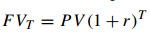
\includegraphics[width=90mm]{figures/formel1-2.png}
\label{fig:formel1-2}
\caption{Formel for compound}
\end{figure}

\textbf{Discount}: Moving money in the opposite direction. A future value of 100 kr at time T has value of 100kr/1.1 = 90.9kr at T-1. This gives us the formula Figure \ref{fig:formel1-3}: 

\begin{figure}[ht!]
\centering
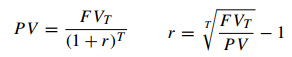
\includegraphics[width=120mm]{figures/formel1-3.png}
\label{fig:formel1-3}
\caption{Formel for discount}
\end{figure}

\subsubsection{Annuities and perpetuities}
Annuity is a series of requal payments at regular time intervals. If we have series of n payments of amount A. If periot interest rate is r, the PV is (right side).

\begin{figure}[ht!]
\centering
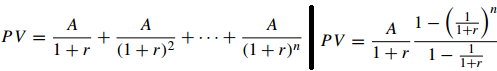
\includegraphics[width=120mm]{figures/formel1-4.png}
\label{fig:formel1-4}
\caption{Formel for annuity}
\end{figure}

We can also discount the individual terms and just get the sum. Sum is (left side). n refers to the number of terms in the series, not discounting periods. Formula calls the first term in the series A/(1+r), whhich in this case does not coincide with the size of annuity. We can then dfine the annuity such that it starts today:

\begin{figure}[ht!]
\centering
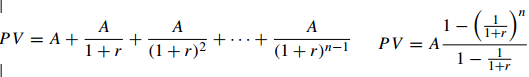
\includegraphics[width=120mm]{figures/formel1-5.png}
\label{fig:formel1-5}
\caption{Formel for annuity too}
\end{figure}

We can use the formula in Fig 4 (left side) to calculate sum of X payment periods. Or Fig 5 (left side) to calucate pay in X amount, one now and one each year the next X years. 

EG if you inherit 1million kr. You get offered 100k each year in 15 years with 10 percent interest. This gives us 836 670, which is less than inheritance. 

How large should annutites each year be in order to equal 1million kr? Just switch PV and A. Use formula with 10percent, we get 119520kr.

For formel Fig 4 (left side, end-of-period annuity), we do this:

\begin{figure}[ht!]
\centering
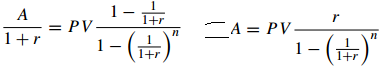
\includegraphics[width=120mm]{figures/formel1-6.png}
\label{fig:formel1-6}
\caption{Formel for compound}
\end{figure}

Amoorization factors are annutites used to pay back a loan with interests.

\textbf{Future value of annuities} can be calculated in the same way. Annutities can be saved so they accumulate future value. Use this formulate to calculate the sum:

\begin{figure}[ht!]
\centering
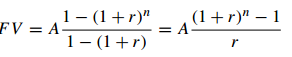
\includegraphics[width=120mm]{figures/formel1-7.png}
\label{fig:formel1-7}
\caption{Formel for compound}
\end{figure}

Future value of 1million kroner today in 15 years is 1000000x1.1opphøydi14 erlik 3797498kr. Using the formula with fifteen payments of 119520 we get the same value.

In order to calculate the annuity given the future value, just move A and FW (A = FV * r / 1+r blabla). If the cost of roof that needs to be replaced in 10 years costs 75k, we need to save 4706 each year with 10percent interest rate.


\textbf{Growing annuties}: Defined as end-of-period payments, but can start immediately. Series of n payments starting today, of amount A what grows with g percent each period. If the period interest rate is r, the present value of annutivy can be written as:

\begin{figure}[ht!]
\centering
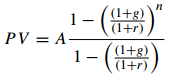
\includegraphics[width=120mm]{figures/formel1-8.png}
\label{fig:formel1-8}
\caption{Formel for compound}
\end{figure}

When annuity starts at the end of the period, we can define first term as blabla, so growth and interest rate factor accumulate over the same number of periods. If the interest rate is 10percent, we have series of five payments that starts with 100kr and grows with 5 percent each year, PV is 415.06.

\begin{figure}[ht!]
\centering
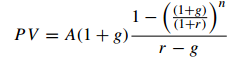
\includegraphics[width=120mm]{figures/formel1-9.png}
\label{fig:formel1-9}
\caption{Formel for compound}
\end{figure}

Future value formula: 

\begin{figure}[ht!]
\centering
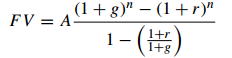
\includegraphics[width=120mm]{figures/formel1-10.png}
\label{fig:formel1-10}
\caption{Formel for compound}
\end{figure}

\textbf{Perpetuities} are annuties with an infinite number of payments. n becomes infinite, as does FV. 

\begin{figure}[ht!]
\centering
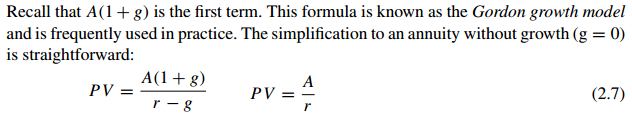
\includegraphics[width=120mm]{figures/formel1-11.png}
\label{fig:formel1-11}
\caption{Formel for compound}
\end{figure}

\subsection{The accounting representation of the firm}
Går litt på det med regnskap. Les senere.

\subsection{An example in investment analysis}
Hvordan bruke forrige delkapittel for å regne ut cash flow.

\subsection{Utility and risk aversion}
Utility is a central concept in economics, it is used to make certain financial decisions.

Risk aversion is the heart of finance and many models are formulated to find the proper price of risk.

Finance studies the choice people make among uncertain future values. Person can prefer good A to B. Preferences are based on what the alternatives means to the people. The concept for that is utility: preferences are described by the notion of utility. When A is preferred to B means that the utility of A is greater than the utility of B.

\begin{figure}[ht!]
\centering
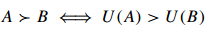
\includegraphics[width=120mm]{figures/formel1-12.png}
\label{fig:formel1-12}
\caption{Formel for compound}
\end{figure}

We can make three simple and general assumptions:
1. People are greedy: they prefer more of a good to less
2. Each additional unit of a good gives less utility than its predecessor.
3. Peoples preferenses are well behaved, meaning they are, among other things: assymetric: if a > b, then b >/= a. Or transitive: if a > b and b>c, then a>c.

The third means that preferences can be expressed in an utility function, that assigns numerical values to a set of choices. Two well-known utility functions are the logarithcmic function and the quadratic: 

\begin{figure}[ht!]
\centering
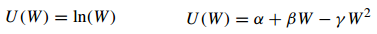
\includegraphics[width=120mm]{figures/formel1-13.png}
\label{fig:formel1-13}
\caption{Formel for compound}
\end{figure}

a, b and y are parameters. W stands for wealth, but can be things like apples, beer, bundle. The logaritmic requires W to be positive, while wealth can be negative. The quadritic is only increasing over a certain range of values of W, up to the "bliss point" W=b/2y where utility is maximal.

Two important concepts can be derived from utility functions: indifference curve and risk aversion.

\textbf{Indifference curves}: represent combinations of choices that gives the same utility. Gives utility as a function of combination of two choices, like saving and consuming.

\textbf{Risk aversion}: implies that a safe 1kr has higher value than a risky 1kr. People require a reward (risk premium) if they take the risk, and are willing to pay insurance to eliminate the risk. For example, if we use quadralitc formula using 

\begin{figure}[ht!]
\centering
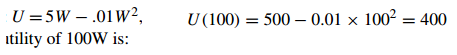
\includegraphics[width=120mm]{figures/formel1-14.png}
\label{fig:formel1-14}
\caption{Formel for compound}
\end{figure}

But what if 100W is not certain, but the expectation of 50W and 100W, each with probability of 50 percent? We can calucate two different things. U(E[W]), utility of expected wealth. Or E[U(W)], expected utility of wealth.

\begin{figure}[ht!]
\centering
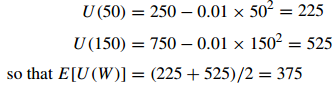
\includegraphics[width=120mm]{figures/formel1-15.png}
\label{fig:formel1-15}
\caption{Formel for compound}
\end{figure}

E[U(W)] is a straight line interpolation between two points U(150) and U(50).







-----


Risk averse - As their wealth increases, their satisfaction or utility increases, but at a decreasing rate. from 1kr to 2kr brings more satisfaction or utility than 20000kr to 20001kr. 

risk neutral - constant marginal utility. 1kr increase in wealth, same increase in utility, is same as 10001 to 10002, utility wase.

risk lover - increasing marginal utility of wealth, more utility as their get wealth. more utility when going from 100001 to 100002. 

